\section{Clan analysis}
\subsection{Clan description}
Met\_repress (CL0057) is a superfamily that contains many antitoxin families, all of which carry a ribbon-helix-helix DNA-binding motif with the beta-ribbon located in and recognizing the major groove of operator DNA\@.

		\subsection{Preprocessing}
Families in clan CL0057 can be separated into 3 groups:
\begin{itemize}
   \item Short (one-domain) unfused unknotted families.
   \item Long (two-domain) fused unknotted families.
   \item Long (two-domain) fused knotted families.
\end{itemize}

Sequences preprocessing steps:
\begin{itemize}
\item Sequences from our clan were downloaded from Pfam, filtered by length, and by similarity, using Cd-Hit 90\%.
\item Families: PF07181, PF08870, and PF10802 were also separated into domains (two for each).
\item Families PF07181 and PF10802 were enriched by additional sequences from Uniprot (and separated into two domains).
\item Additionally, we added one more unknotted fusion sequence from PDB structure 4hv0. (Described as PF00000) (Discussion?)
\end{itemize}

      \subsection{CLANS}
The problem here was that many Pfam families didn't cluster into families, and instead, produced ''cloud''.
There are no clear borders between many families.
On the other hand, there were also families located quite far from others.
To solve ''cloud'' problems, we tried two solutions.
Alternative clustering using MCL\@.
Because separating sequences based on families failed, the idea was to create alternative clusters based on sequence similarity (BLAST).
We tried various parameter values from 1.1 (too large clusters) to 6 (massive amount of small clusters (1-2 sequences)) with the best results using values between 1.4-1.5.
Unfortunately, while MCL presented slightly better clusters, even then sequences were mixed between clusters.
Similarly, we tried using several different methods - both sequence and statistically based without success.
All methods were classifying the main cloud as one-two clusters or many groups without clear borders.
Instead, we tried clearing sequences even further while using standard family-based separation.
So we used Cd-Hit again, this time with lower percentage values.
We were using one or two-step filtering.
The first part was to run Cd-Hit 50\% clusters, and instead of taking output sequences (such filtering would be too strict), we deleted clusters with 1--2 sequences only.
If there were still problems with clustering, we were rerunning Cd-Hit 70\% and again deleted only small clusters with up to 3--4 sequences.
Such a process is reducing the outer part of the CLANS clusters - sequences mostly invalid or different from the rest while leaving core, family representative sequences mostly untouched.
This approach gave much better results - the ''cloud'' was still there, but much cleaner.


        \subsubsection{Cloud problem}
\begin{itemize}
   \item MCL clustering - no desired effects.
   \begin{itemize}
      \item Parameters tested from 1.1 to 6.
      \item Best values - around 1.4-1.5 - Still clusters were mixed and didn't solve
   \end{itemize}
   \item Reducing the number of sequences using Cd-Hit with a lower percentage: 50--80\% (Depending on the family).
      This partially solved the problem as the cloud was slightly more clearer, however, it didn't completely separate families.
\end{itemize}


\begin{figure}[H]
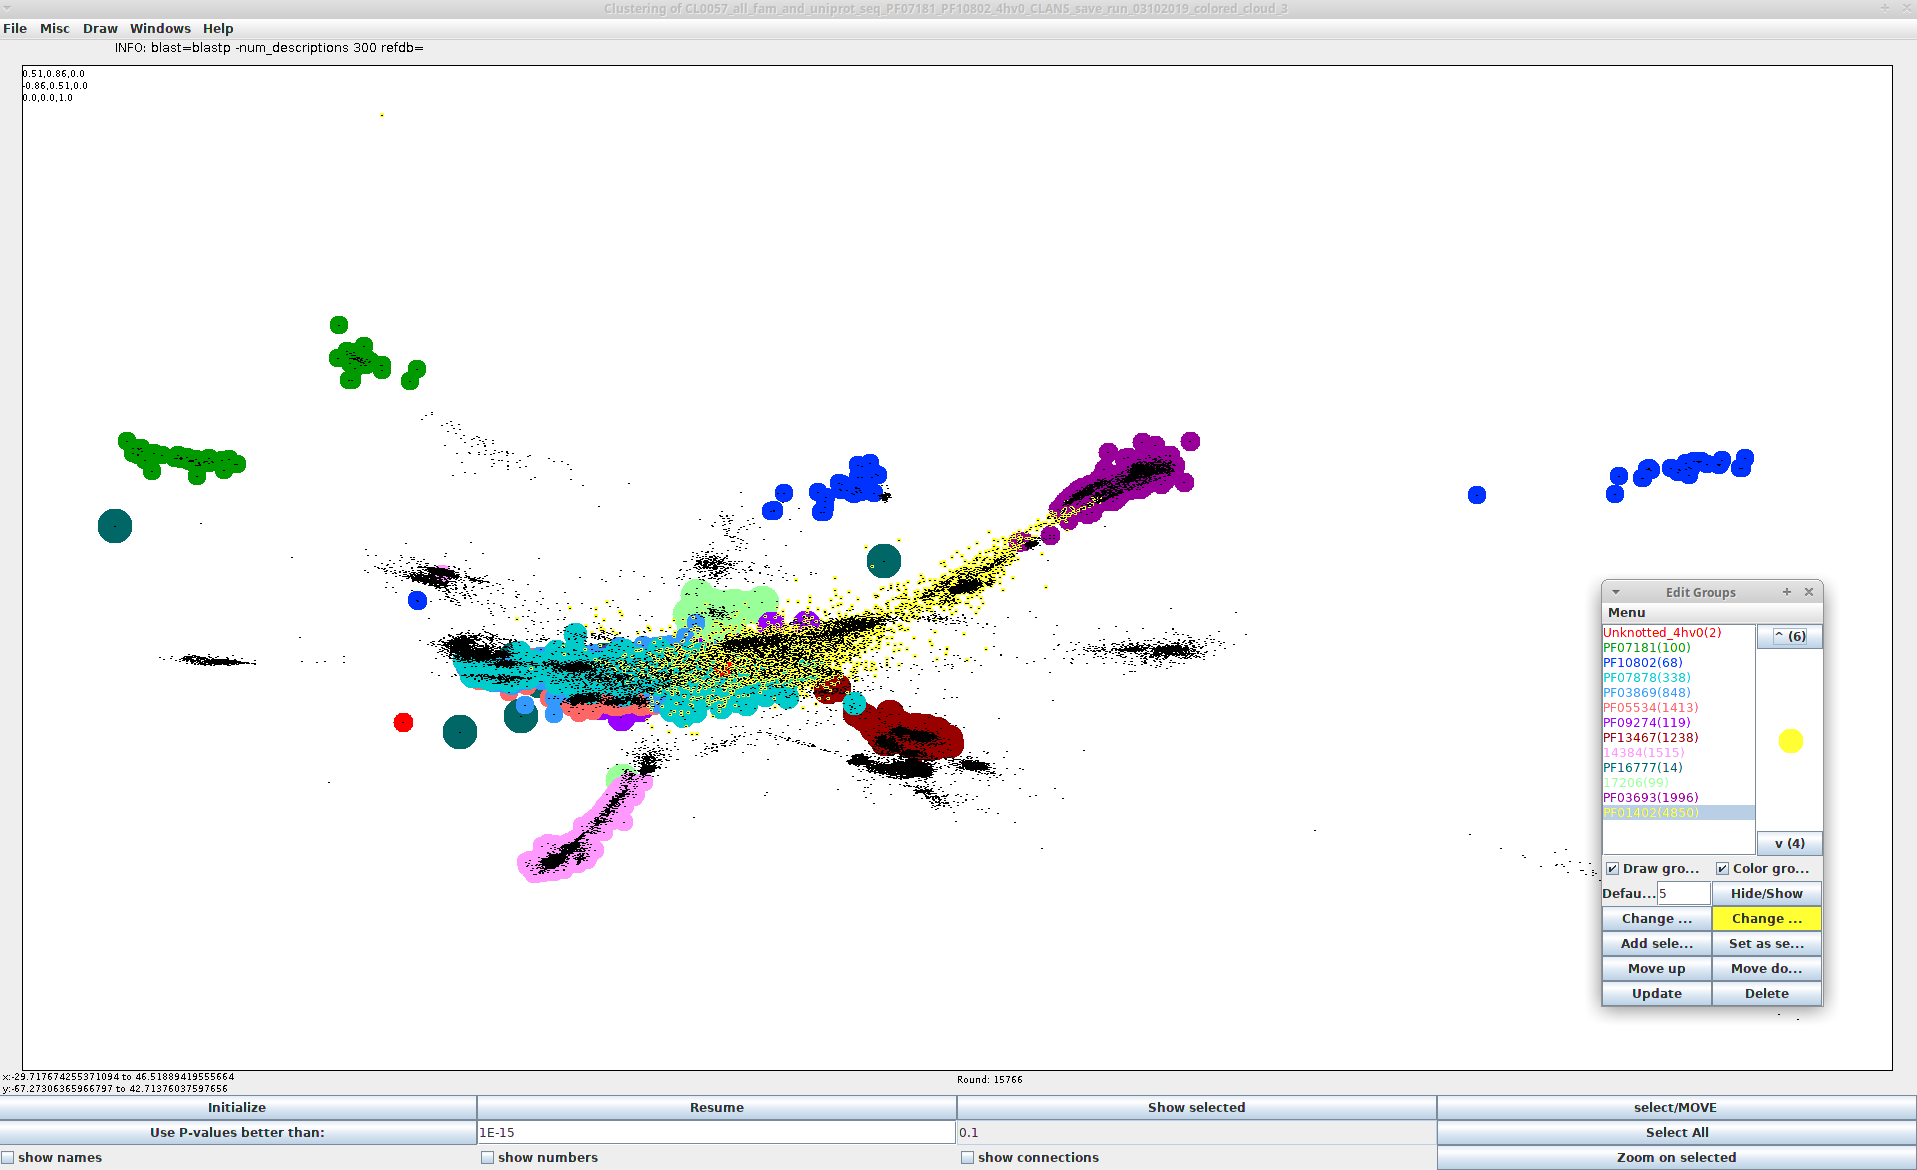
\includegraphics[width=\textwidth]{CLANS_1_2}
\caption{CL0057 clustering in CLANS. Family PF08870 is missing ($\sim$300 seq).}
\end{figure}

      \subsection{Ola's Workflow, profiles}
Two families were ignored by workflow because of their e-value bigger than 0.01.
Another test shows that those two families were also much different from each other.

\begin{figure}[H]
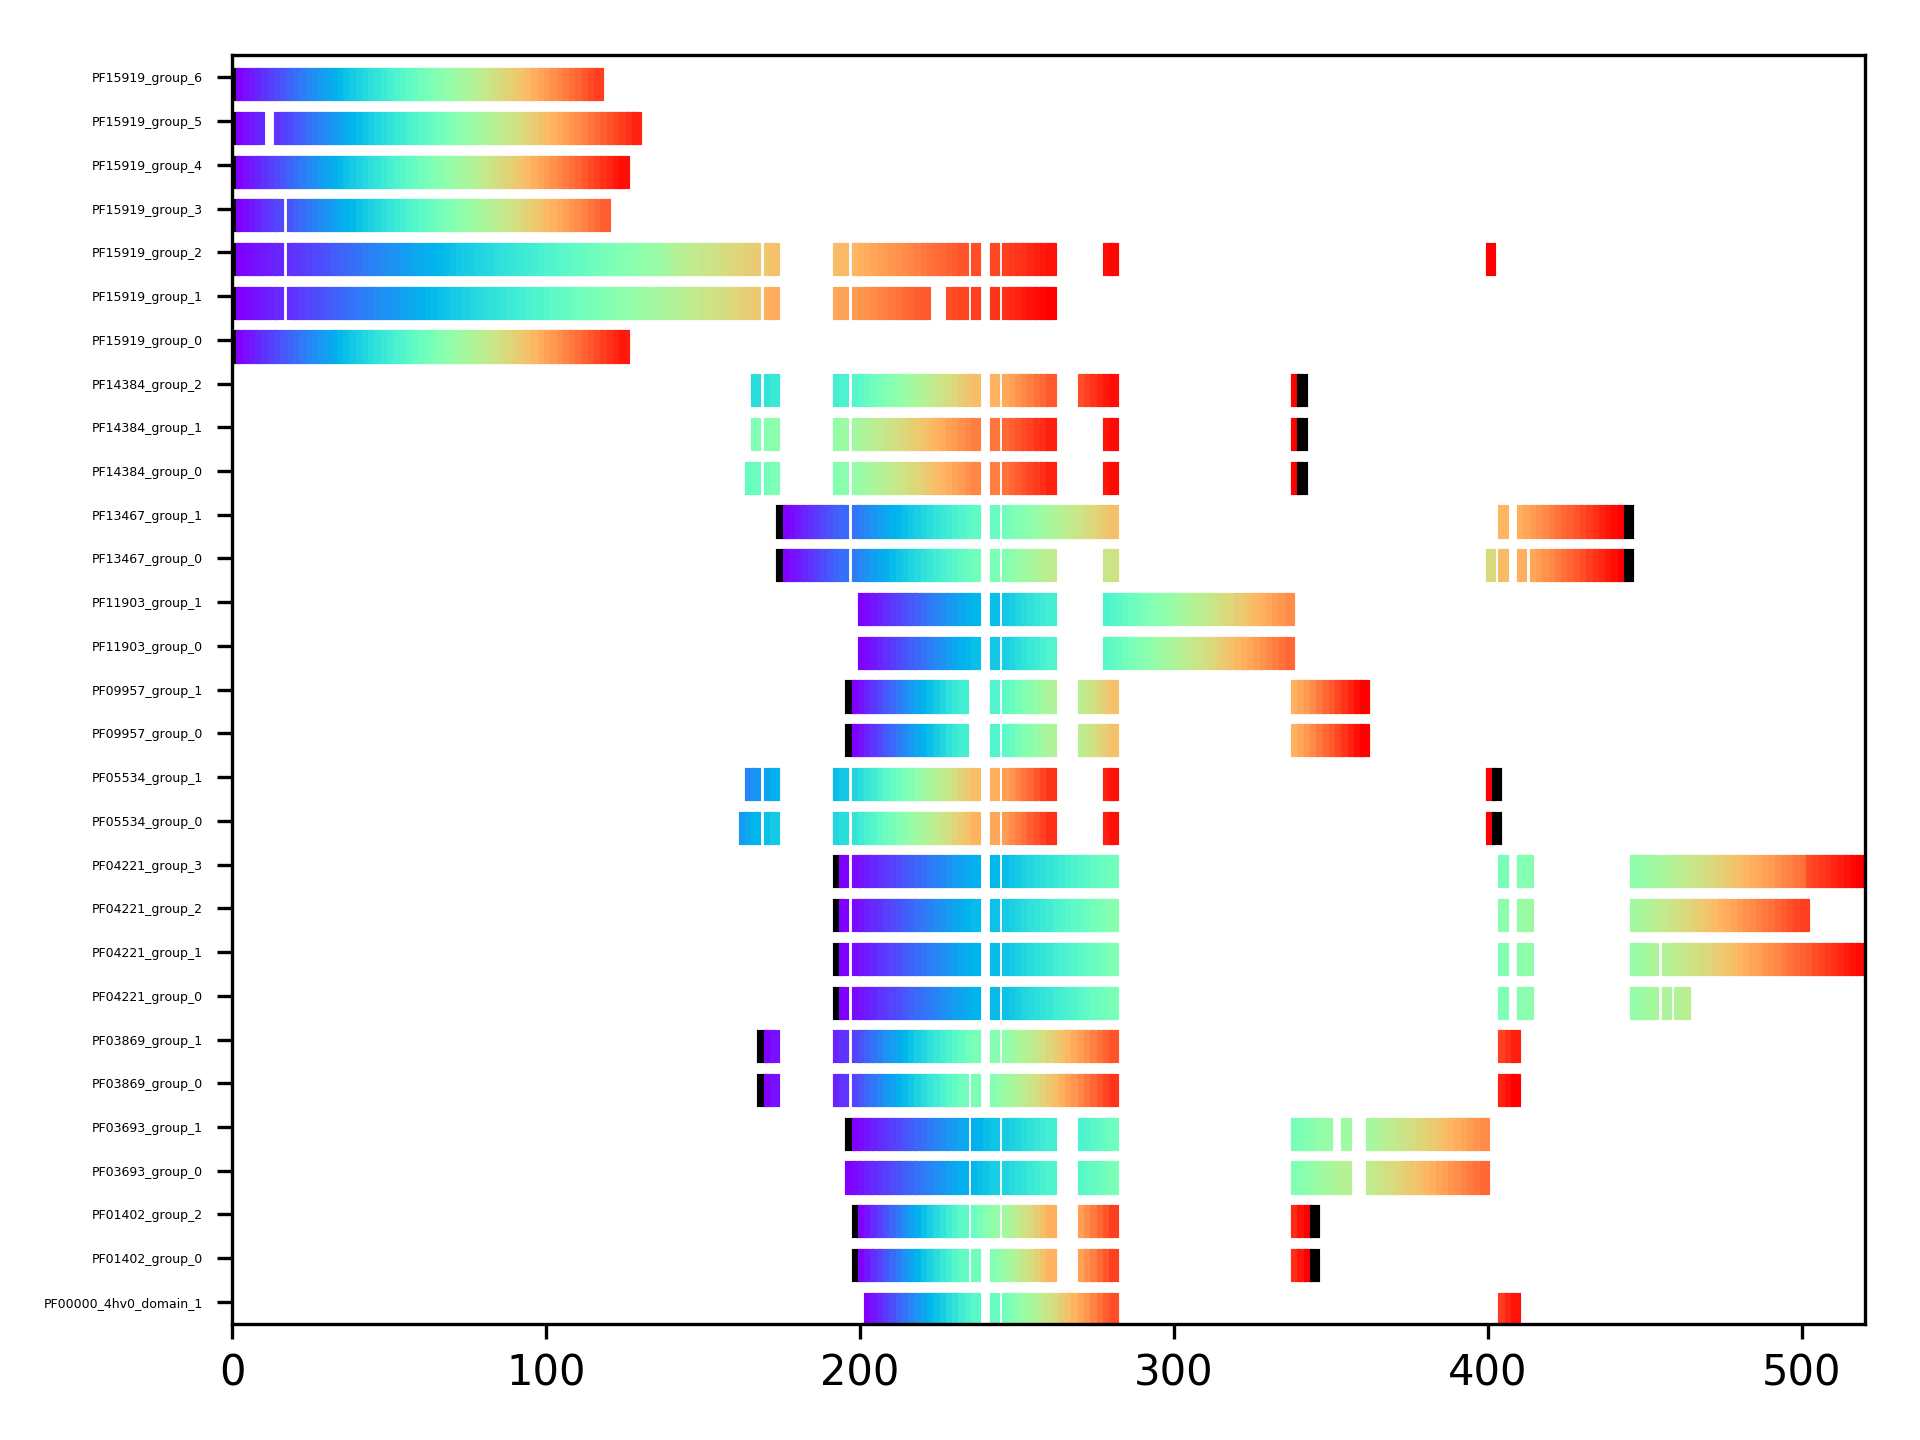
\includegraphics[width=0.8\textwidth]{cuddly_1}
\caption{Plot from Ola's Workflow with families from clan CL0057.}
\end{figure}

\begin{figure}[H]
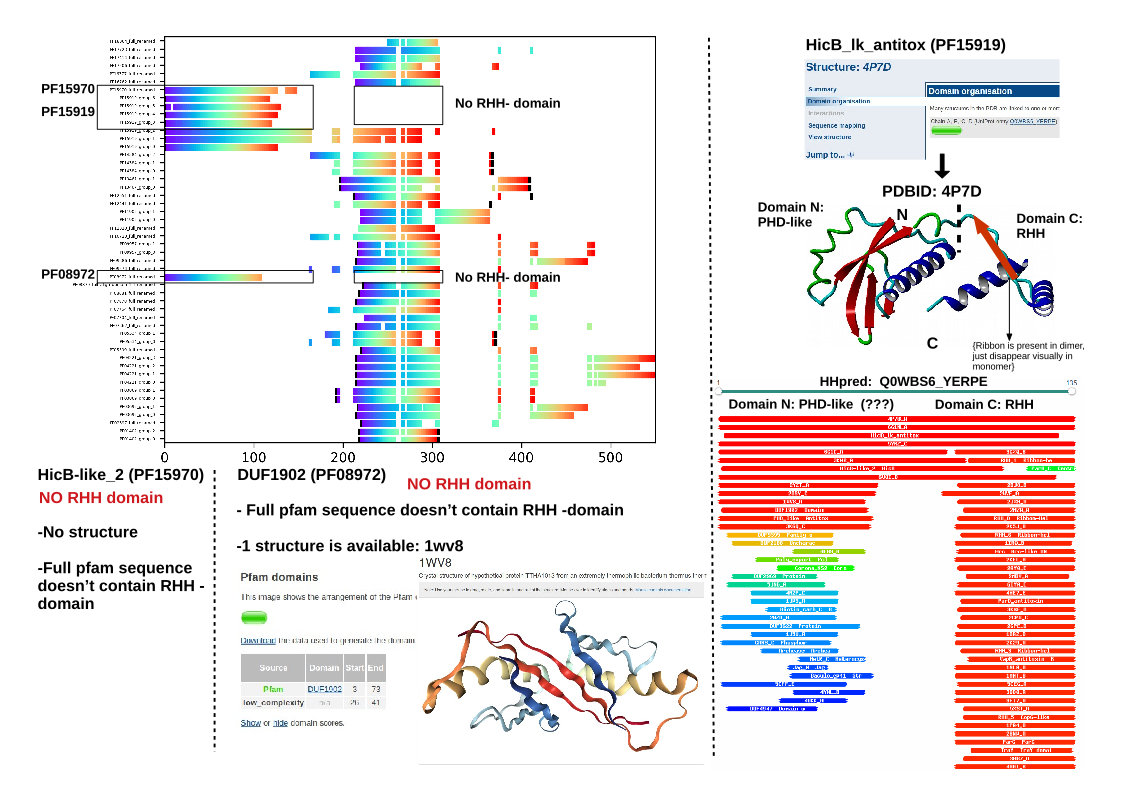
\includegraphics[width=0.8\textwidth]{cuddly_2}
\caption{Clan CL0057 domain analysis.}
\end{figure}

        \subsection{Clan trees}
I decided to start by creating a tree with families from our clan only to tune parameters.
There was some progress from ''brush'' only trees to much better-looking ones.
However, their quality was far from perfect, so I consider this part as not finished yet.

\begin{figure}[H]
\begin{center}
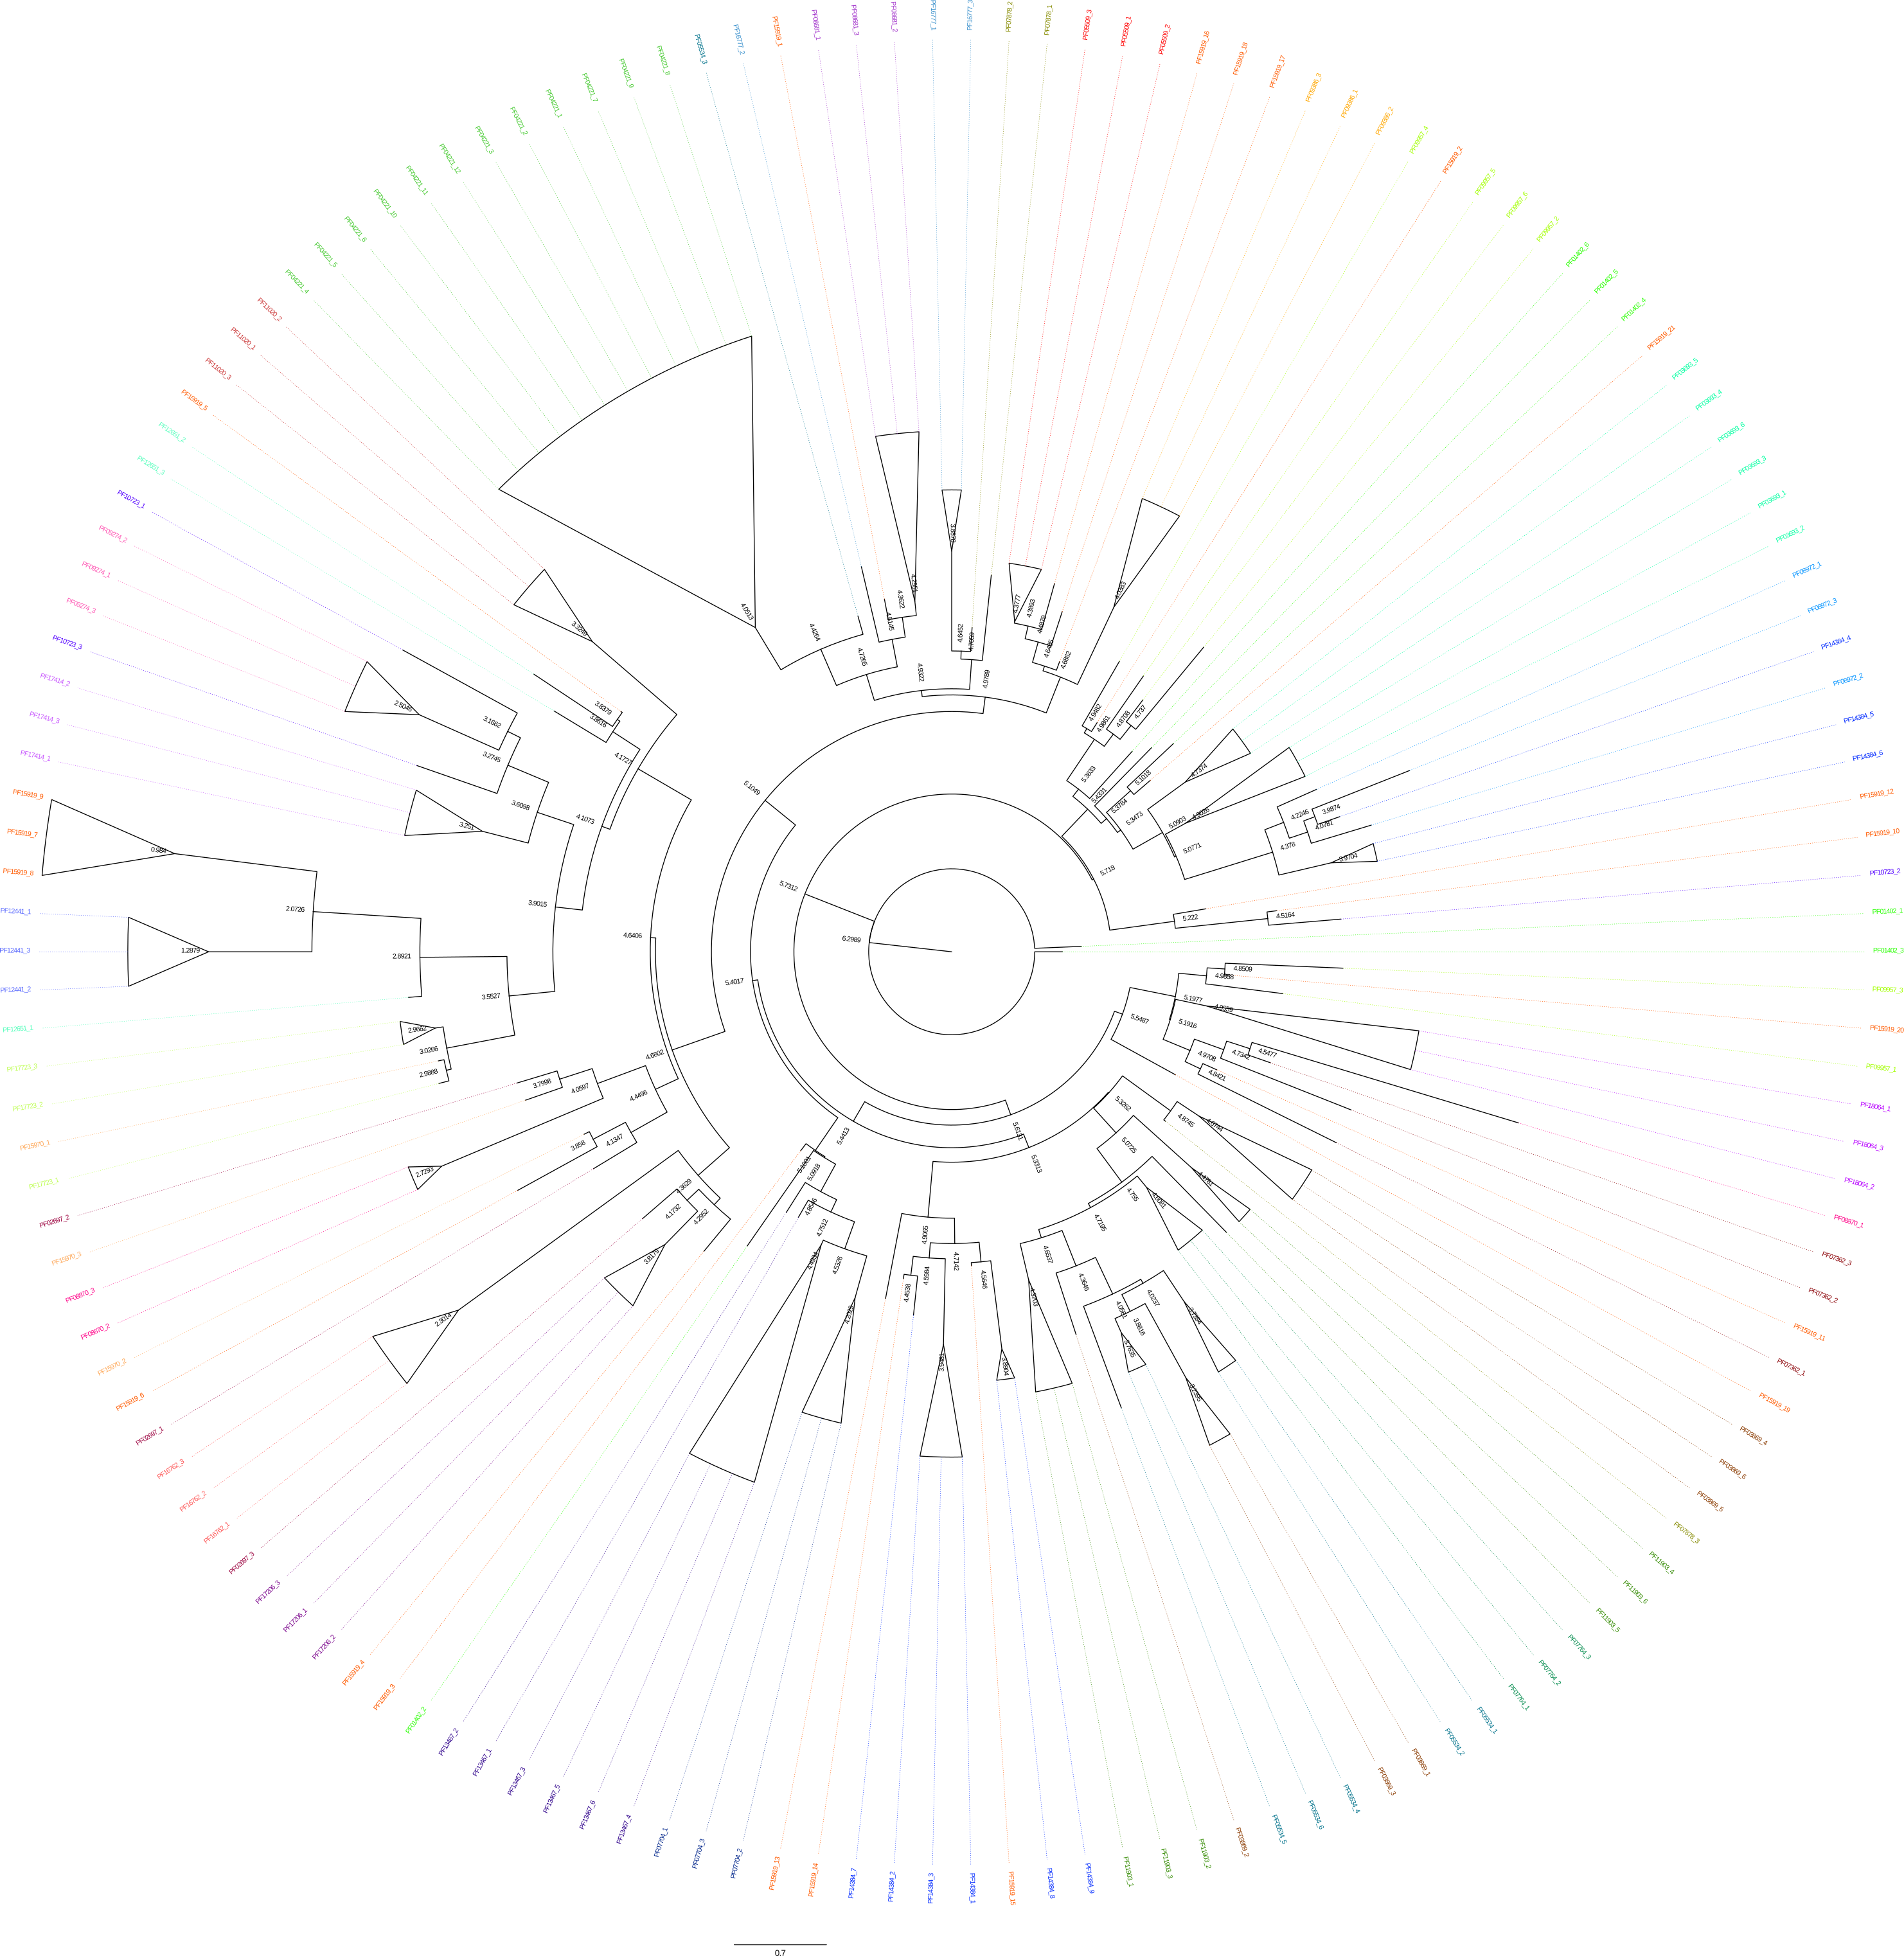
\includegraphics[width=0.5\textwidth]{tree_1}
\caption{Best old tree.}
\end{center}
\end{figure}


    \subsubsection{Automatic model selection tools}
\begin{itemize}
    \item SMS: Both AIC and BIC criterium are suggesting Vt +G+F model.
    \item IQTREE model finder - VT
    \item MrBayes - Blosum
\end{itemize}


    \subsubsection{First tree}
    Preprocessing:
    \begin{itemize}
        \item Families listed above were downloaded from Pfam (domains, full, unaligned)
        \item Reduced using Cd-Hit 80\%
        \item Renamed using script.
    \end{itemize}


    \subsubsection{Best tested trees}
In the results below tree calculated using 4 chains reached 0.016 SD and using 12 chains - 0.022 (goal is to reach 0.01 or lower, while range 0.01-0.05 is acceptable).
PSRF (Possible Scale Reduction Factor) values were around 0.9998 (So very close to target: 1)
However, those values probably can still be improved after more generations.

\begin{figure}[H]
\begin{center}
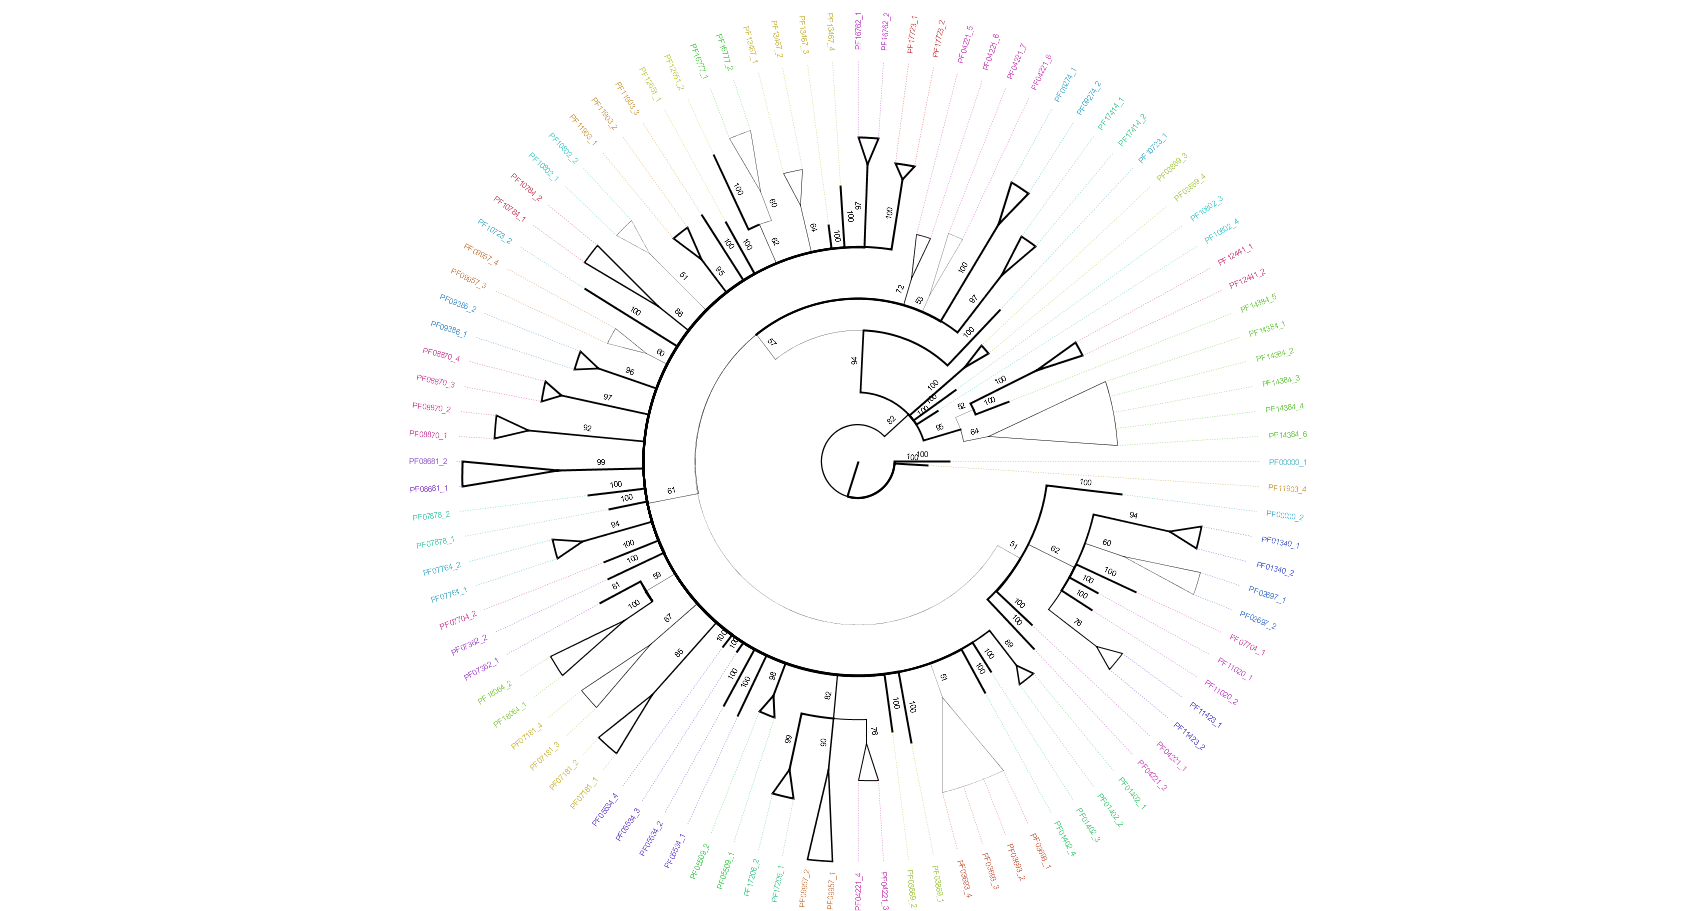
\includegraphics[width=0.9\textwidth]{4_ch_tree.png}
\caption{4 chains long run tree.}
\end{center}
\end{figure}

\begin{figure}[H]
\begin{center}
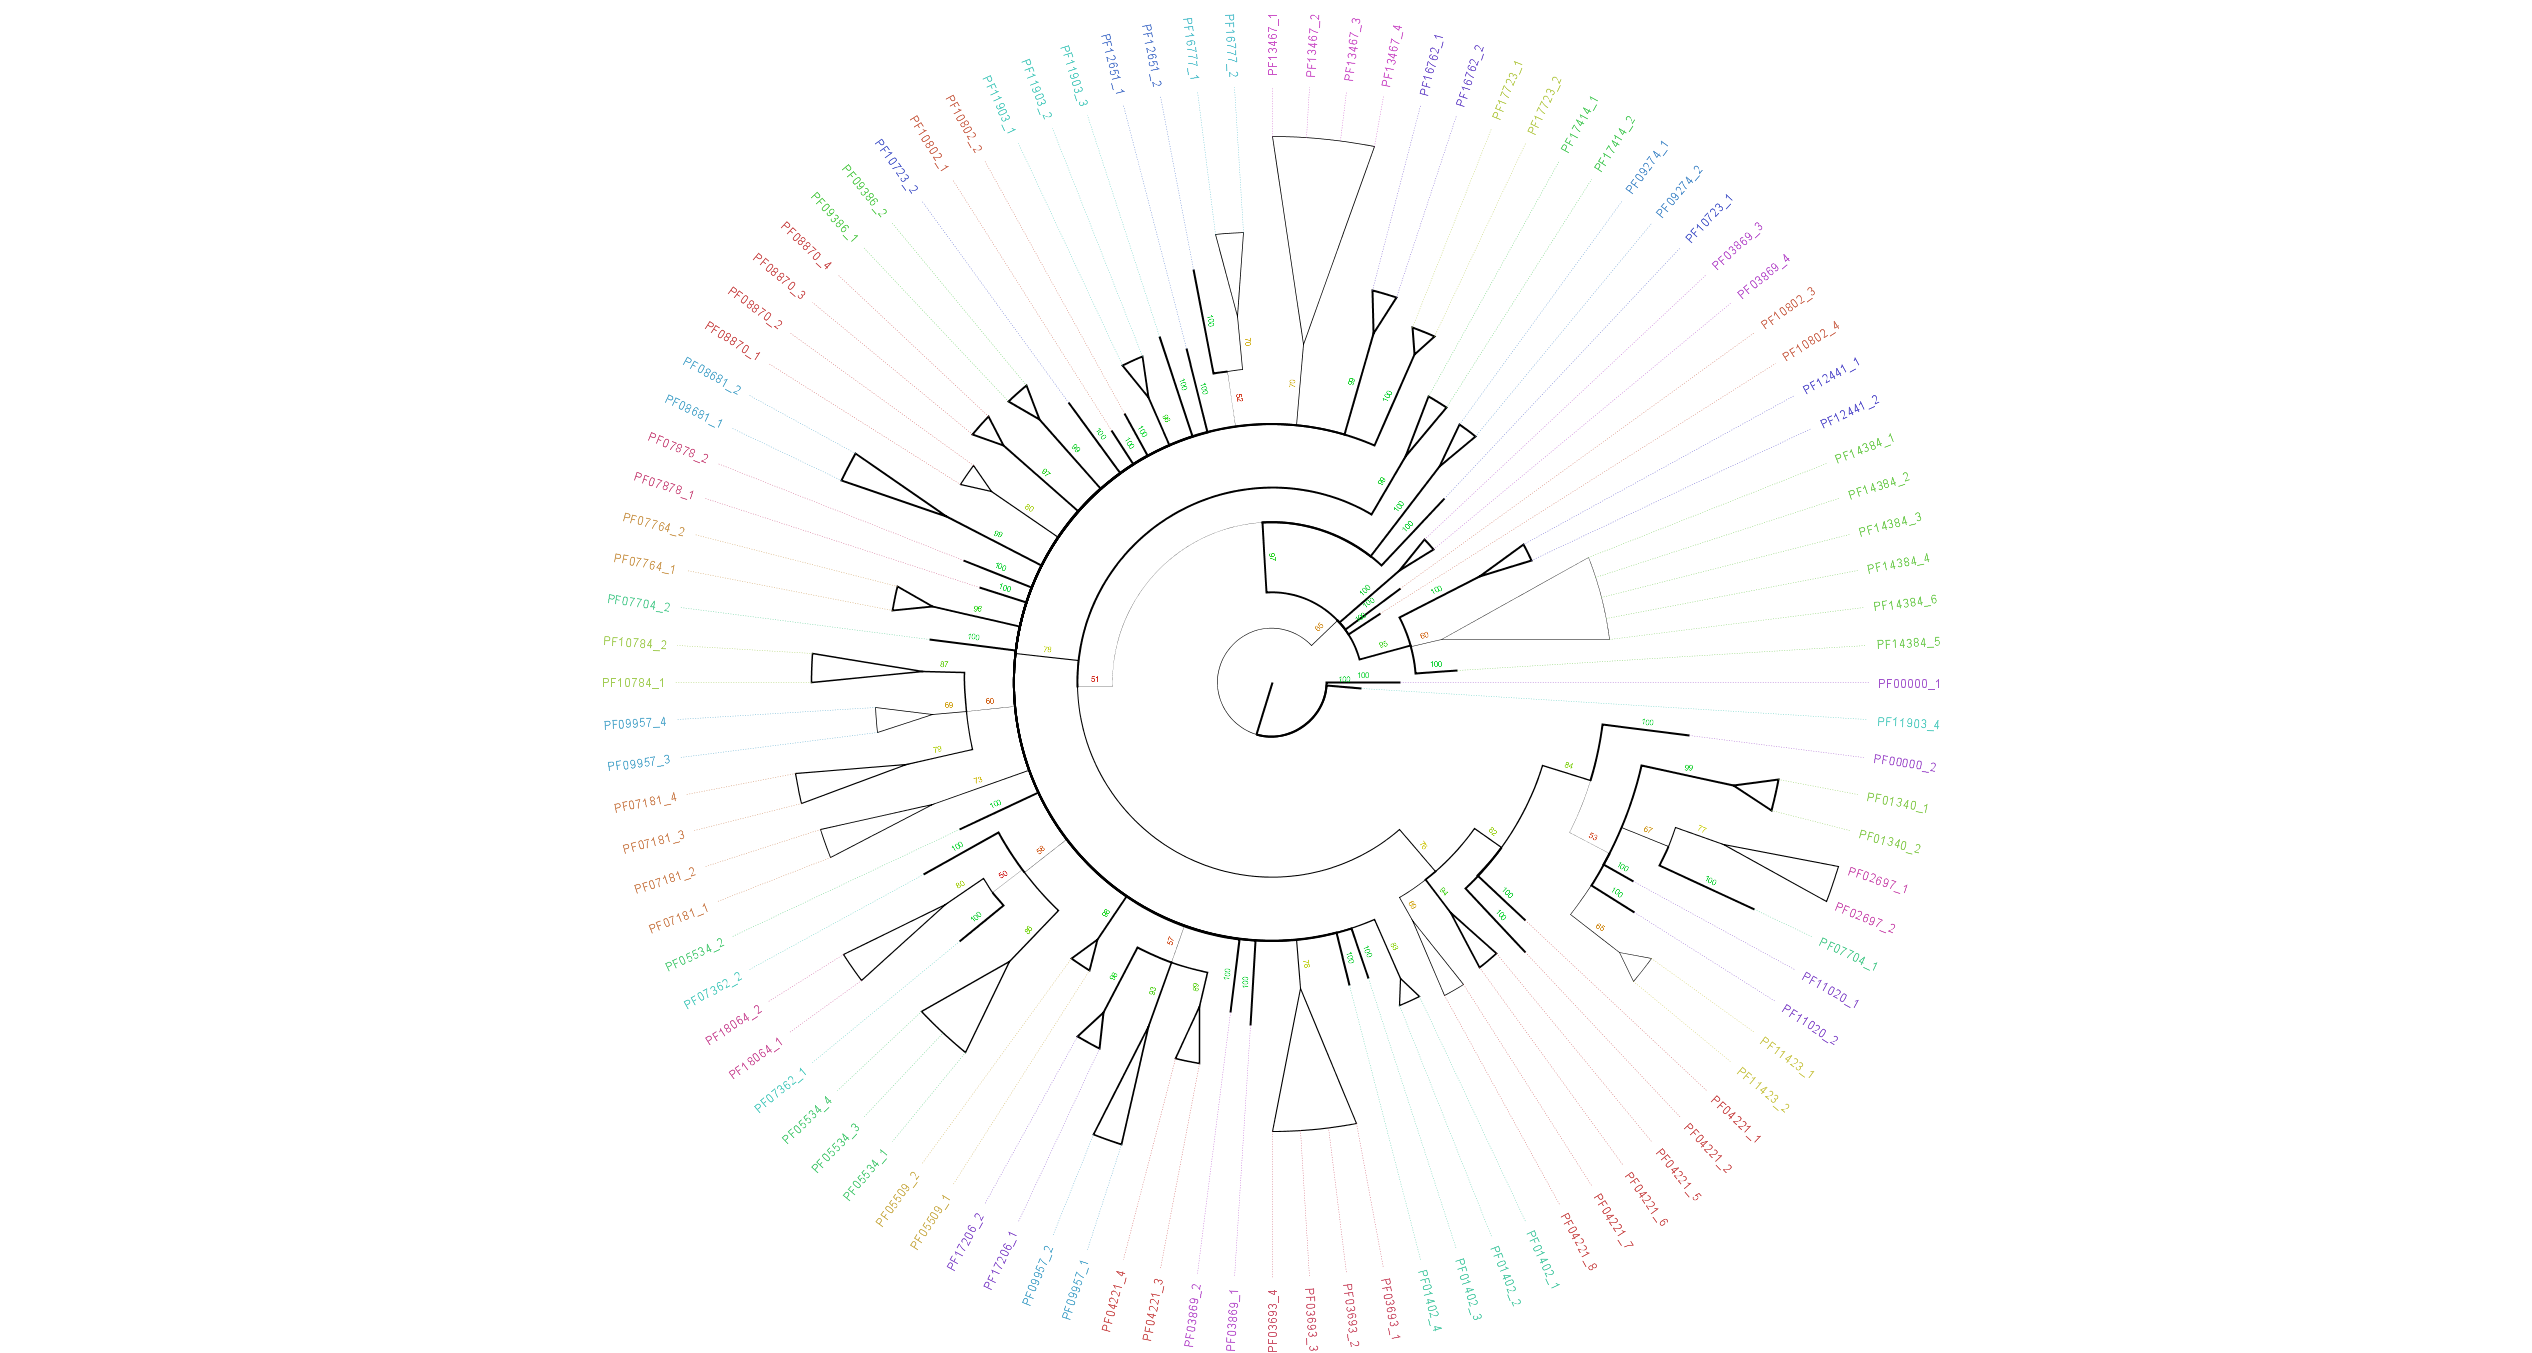
\includegraphics[width=0.9\textwidth]{12_ch_tree.png}
\caption{12 chains short run tree.}
\end{center}
\end{figure}

\begin{figure}[H]
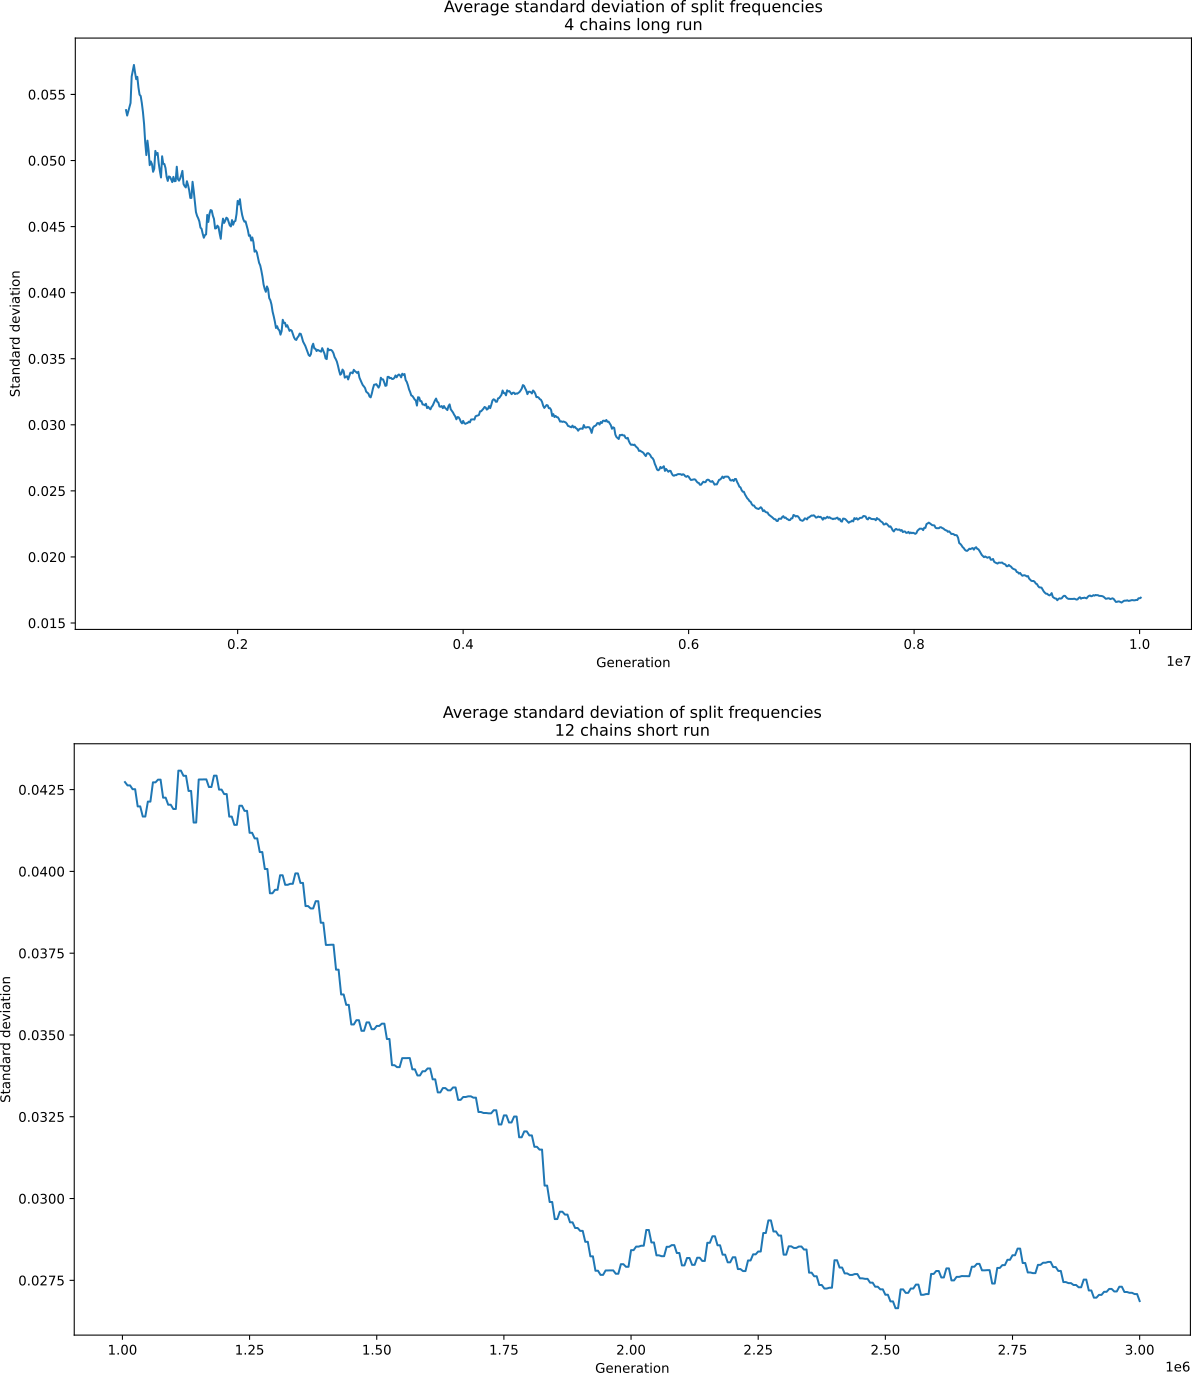
\includegraphics[width=\textwidth]{sd_plots.png}
\caption{The average standard deviation of split frequencies during both runs. Trees are trying to reach 0.01 values, however, 0.01-0.05 is still acceptable. Plots are starting from 1.000.000 generation. Notice, that 4 chains run has 10.000.000 generations while 12 chains run only 3.000.000.}
\end{figure}